\item \defpoints{20} [Decision Tree] A dataset is given below. Now we want to discover the relationship between the features and the target variable by using a Decision Tree.
\
\begin{table*}[h]
    \centering
    \begin{tabular}{|c|c|c|c|}
        \hline
        Outlook $\left(X_{1}\right)$ & Temperature $\left(X_{2}\right)$ & Humidity $\left(X_{3}\right)$ & Play Tennis? $(Y)$ \\
        \hline
        sunny & hot & high & no \\
        \hline
        overcast & hot & high & yes \\
        \hline
        rain & mild & high & yes \\
        \hline
        rain & cool & normal & yes \\
        \hline
        sunny & mild & high & no \\
        \hline
        sunny & mild & normal & yes \\
        \hline
        rain & mild & normal & yes \\
        \hline
        overcast & hot & normal & yes \\
        \hline
    \end{tabular}
\end{table*}

\begin{enumerate}
    \item Using the dataset above, calculate the mutual information for each feature ($X_{1}, X_{2}, X_{3}$) to determine the root node for a Decision Tree trained on the above data.
    \begin{itemize}
        \item What is $I\left(Y ; X_{1}\right)$? \defpoints{3}
        \item What is $I\left(Y ; X_{2}\right)$? \defpoints{3}
        \item What is $I\left(Y ; X_{3}\right)$? \defpoints{3}
        \item What feature should be split on at the root node? \defpoints{1}
    \end{itemize}

    \item Calculate what the next split should be. \defpoints{5}

    \item Draw the resulting tree. \defpoints{5}
\end{enumerate}

\solution

(a) $$\mathrm{H}(\mathrm{Y})=-\frac{6}{8} * \log _{2}\left(\frac{6}{8}\right)-\frac{2}{8} * \log _{2}\left(\frac{2}{8}\right) \approx 0.811 $$
\begin{itemize}
    \item $I\left(Y ; X_{1}\right)=0.467$ \\
    For attribute $X_{1}$,
    \begin{align*}
    & -H\left(Y \mid X_{1}=\text { sunny }\right)=-\left[\frac{1}{3} * \log _{2}\left(\frac{1}{3}\right)+\frac{2}{3} * \log _{2}\left(\frac{2}{3}\right)\right] \approx 0.918 \\
    & -H\left(Y \mid X_{1}=\text { rain }\right)=0 \\
    & -H\left(Y \mid X_{1}=\text { overcast }\right)=0 \\
    & \Rightarrow H\left(Y \mid X_{1}\right)=\left[\frac{3}{8} * 0.918+\frac{3}{8} * 0+\frac{2}{8} * 0\right] \approx 0.344 \\
    & \Rightarrow I\left(Y ; X_{1}\right) \approx 0.811-0.344=0.467
    \end{align*}

    \item $I\left(Y ; X_{2}\right)=0.061$\\
    For attribute $X_{2}$,
    \begin{align*}
    & -H\left(Y \mid X_{2}=\text { hot }\right)=-\left[\frac{1}{3} * \log _{2}\left(\frac{1}{3}\right)+\frac{2}{3} * \log _{2}\left(\frac{2}{3}\right)\right] \approx 0.918 \\
    & -H\left(Y \mid X_{2}=\text { cool }\right)=0 \\
    & -H\left(Y \mid X_{2}=\text { mild }\right)=-\left[\frac{3}{4} * \log _{2}\left(\frac{3}{4}\right)+\frac{1}{4} * \log _{2}\left(\frac{1}{4}\right)\right] \approx 0.811 \\
    & \Rightarrow H\left(Y \mid X_{2}\right)=\left[\frac{3}{8} * 0.918+\frac{1}{8} * 0+\frac{4}{8} * 0.811\right] \approx 0.75 \\
    & \Rightarrow I\left(Y ; X_{2}\right) \approx 0.811-0.75=0.061
    \end{align*}
    \item $I\left(Y ; X_{3}\right)=0.311$\\
    For attribute $X_{3}$,\\
    \begin{align*}
    & -H\left(Y \mid X_{3}=\text{high}\right)=-\left[\frac{1}{2} * \log _{2}\left(\frac{1}{2}\right)+\frac{1}{2} * \log _{2}\left(\frac{1}{2}\right)\right]=1\\
    & -H\left(Y \mid X_{2}=\text{normal}\right)=0\\
    & \Rightarrow H\left(Y \mid X_{3}\right)=\left[\frac{4}{8} * 1.0+\frac{4}{8} * 0\right]=0.5\\
    & \Rightarrow I\left(Y ; X_{3}\right) \approx 0.811-0.5=0.311
    \end{align*}

    \item Split on $X_{1}$ at the root node\\
    Since splitting on attribute $X_{1}$ gives the highest mutual information, the root node is $X_{1}$.
\end{itemize}


(b) From the above part, as we can see that the sub-datasets $\mathcal{D}_{\left(X_{1}=\text { rain }\right)}$ and $\mathcal{D}_{\left(X_{1}=\text { overcast }\right)}$ are pure, there will be no further splitting on those and we will place a leaf node with label assignment decided by majority vote classifier. So, we need to split only on the sub-dataset $\mathcal{D}_{\left(X_{1}=\text { sunny }\right)}$. Now, we will use only $\mathcal{D}_{\left(X_{1}=\text { sunny }\right)}$ to estimate the probabilities for the next split.\\
$H(Y)=-\frac{1}{3} * \log _{2}\left(\frac{1}{3}\right)-\frac{2}{3} * \log _{2}\left(\frac{2}{3}\right) \approx 0.918$\\
For attribute $X_{2}$,
\begin{itemize}
    \item $H\left(Y \mid X_{2}=h o t\right)=0$
    \item $H\left(Y \mid X_{2}=\operatorname{cool}\right)=0$
    \item $H\left(Y \mid X_{2}=\right.$ mild $)=-\left[\frac{1}{2} * \log _{2}\left(\frac{1}{2}\right)+\frac{1}{2} * \log _{2}\left(\frac{1}{2}\right)\right]=1$\\
$\Rightarrow H\left(Y \mid X_{2}\right)=\left[\frac{2}{3} * 1.0+\frac{1}{3} * 0\right] \approx 0.67$\\
$\Rightarrow I\left(Y ; X_{2}\right) \approx 0.918-0.67 \approx 0.25$\\
\end{itemize}
For attribute $X_{3}$,
\begin{itemize}
    \item $H\left(Y \mid X_{3}=h i g h\right)=0$
    \item $H\left(Y \mid X_{3}=\right.$ normal $)=0$\\
$\Rightarrow H\left(Y \mid X_{3}\right)=\left[\frac{2}{3} * 0+\frac{1}{3} * 0\right]=0$\\
$\Rightarrow I\left(Y ; X_{3}\right) \approx 0.918$
\end{itemize}
We split using attribute $X_{3}$ as it gives the highest mutual information.


(c) \\
\begin{figure}[h!] % h表示这里(Here)插入
    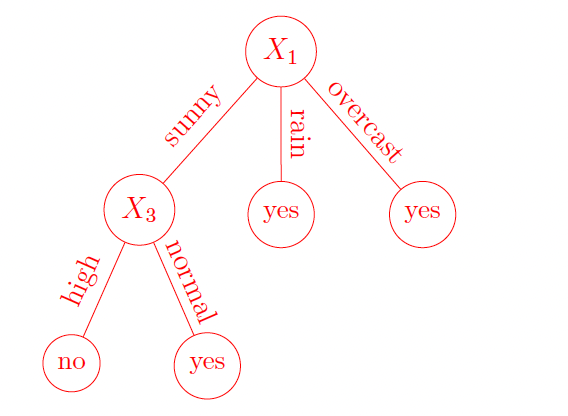
\includegraphics[width=0.5\textwidth]{./DT-3.png} % 设定图片宽度为页面宽度的一半
    \label{fig:DT-3} % 图片标签(用于引用)
\end{figure}

\newpage